\documentclass[10pt,twocolumn]{article}
\usepackage[margin=0.72in]{geometry}
\usepackage{mathptmx}
\usepackage{amsmath,amssymb}
\usepackage{booktabs}
\usepackage{graphicx}
\usepackage{titlesec}
\usepackage[table,dvipsnames]{xcolor}
\usepackage{microtype}
\usepackage{caption}
\usepackage{pifont}
\usepackage{tikz}
\usetikzlibrary{arrows.meta,positioning,calc,fit,backgrounds,shapes.geometric}
\usepackage[hidelinks]{hyperref}

\captionsetup{font=small,labelfont=bf,skip=4pt}
\titleformat{\section}{\normalfont\large\bfseries}{\thesection}{0.6em}{}
\titleformat{\subsection}{\normalfont\normalsize\bfseries}{\thesubsection}{0.6em}{}
\titlespacing*{\section}{0pt}{1.35ex plus .3ex}{0.7ex}
\titlespacing*{\subsection}{0pt}{1.0ex plus .2ex}{0.5ex}
\newcommand{\code}[1]{\texttt{\small #1}}
\setlength{\parskip}{0.15ex}
\pagestyle{empty}

% ---- palette (muted, publication-grade) ----
\definecolor{cExpLn}{HTML}{C0452F}\definecolor{cExpBg}{HTML}{FBEAE5}
\definecolor{cChpLn}{HTML}{2E6DA4}\definecolor{cChpBg}{HTML}{E6EFF8}
\definecolor{cDecLn}{HTML}{3C8B57}\definecolor{cDecBg}{HTML}{E7F2EB}
\definecolor{cAuxLn}{HTML}{8A8A8A}\definecolor{cAuxBg}{HTML}{F0F0F0}
\definecolor{cStLn}{HTML}{45566A}\definecolor{cStBg}{HTML}{EDF1F5}
\definecolor{cAmbLn}{HTML}{B07A10}\definecolor{cAmbBg}{HTML}{FBF2DD}
\definecolor{cZone}{HTML}{F7F5EF}\definecolor{cZoneLn}{HTML}{CFC7B3}
% ---- shared TikZ styles ----
\tikzset{
  box/.style={rectangle, rounded corners=2.6pt, draw=black!70, line width=0.7pt,
              align=center, inner sep=3.4pt, font=\scriptsize, minimum height=8.5mm},
  exp/.style={box, fill=cExpBg, draw=cExpLn, text=black!88},
  chp/.style={box, fill=cChpBg, draw=cChpLn, text=black!88},
  dec/.style={box, fill=cDecBg, draw=cDecLn, text=black!88},
  aux/.style={box, fill=cAuxBg, draw=cAuxLn, dashed, text=black!70},
  st/.style={box, fill=cStBg, draw=cStLn},
  cache/.style={box, fill=white, draw=black!45, densely dashed},
  lgd/.style={draw, rounded corners=1.4pt, line width=0.7pt, minimum width=4.2mm, minimum height=2.6mm, inner sep=0pt},
  a/.style={-{Stealth[length=4.6pt,width=3.6pt]}, line width=0.7pt, draw=black!72},
  ax/.style={-{Stealth[length=4.6pt,width=3.6pt]}, line width=0.9pt, draw=cExpLn},
  ac/.style={-{Stealth[length=4.6pt,width=3.6pt]}, line width=0.9pt, draw=cChpLn},
  ad/.style={-{Stealth[length=4.2pt,width=3.2pt]}, line width=0.7pt, draw=cAuxLn, dashed},
  loop/.style={-{Stealth[length=4.6pt,width=3.6pt]}, line width=0.7pt, draw=black!55, densely dotted}
}

\begin{document}
\twocolumn[
\begin{center}
{\LARGE\bfseries What Actually Helps a Training-Free\\[2pt]
Diffusion Predictor? A Falsification Study of\\[2pt]
Token-Adaptive Prediction on an Exact-Residual Testbed\par}
\vspace{10pt}
{\large Bhavith Chandra Challagundla\par}
\vspace{3pt}
{\small New York University \;\textbullet\; \href{https://Bhavith-Chandra.github.io}{Bhavith-Chandra.github.io}\par}
\vspace{13pt}
\begin{minipage}{0.88\textwidth}
\small
\textbf{Abstract.} Training-free diffusion accelerators such as the Token-Adaptive
Predictor (TAP) reconstruct skipped network outputs from cached features, selecting per
token which cheap predictor to trust by reading a first-layer \emph{probe} and ranking
predictors with a cosine proxy. We investigate three candidate improvements suggested by a
single-seed pilot: an $L_2$ proxy in place of cosine, online least-squares predictors in
place of fixed Taylor extrapolators, and the probe's per-token adaptivity. Using an
exact-residual Gaussian-mixture testbed, in which the true denoiser output is available in
closed form (Tweedie) and proxy fidelity is therefore directly measurable without a trained
network, we conduct a $12$-seed core study, a $21$-regime sweep, and a pre-registered
$30$-test adversarial suite, all with bootstrap $95\%$ confidence intervals. The results
are largely negative. (i) The $L_2$ proxy improves rank fidelity in all $21$ regimes, but
the effect is small ($\Delta$Spearman $+0.016$, CI $(+0.014,+0.019)$) rather than the
roughly fourfold gain observed in the pilot, and increases only as the task becomes harder.
(ii) Online predictors do not outperform fixed Taylor extrapolators; they are consistently
worse, in $19$ of $21$ regimes. (iii) Probe-then-select surpasses a strong fixed predictor
only under aggressive acceleration, so at moderate speedups the acceleration alone, not the
adaptivity, accounts for the observed gains. We further show that per-token selection is
already optimal: the objective is separable, equal-cost, and unconstrained, so greedy
selection attains the global optimum. This reframes the central quantity as \emph{proxy
fidelity}, since an oracle selector retains headroom that the probe cannot capture and
fidelity increases monotonically with probe richness (from $0.33$ to $1.0$). We also explain
why an $L_2$ proxy tracks the $L_2$ output residual more faithfully than a magnitude-blind
cosine.\par
\vspace{4pt}
\textit{TAP (arXiv:2603.03792) provides no public implementation; all TAP behaviour reported
here rests on a faithful reimplementation. The testbed is a shallow analytic denoiser and
does not include the deep learned layers that make a real first-layer probe more
informative; we quantify this gap rather than leave it implicit. All code and numerical
results are released.}
\end{minipage}
\end{center}
\vspace{9pt}
]

% =========================== ARCHITECTURE DIAGRAM ===========================
\begin{figure*}[t]\centering
\resizebox{\textwidth}{!}{%
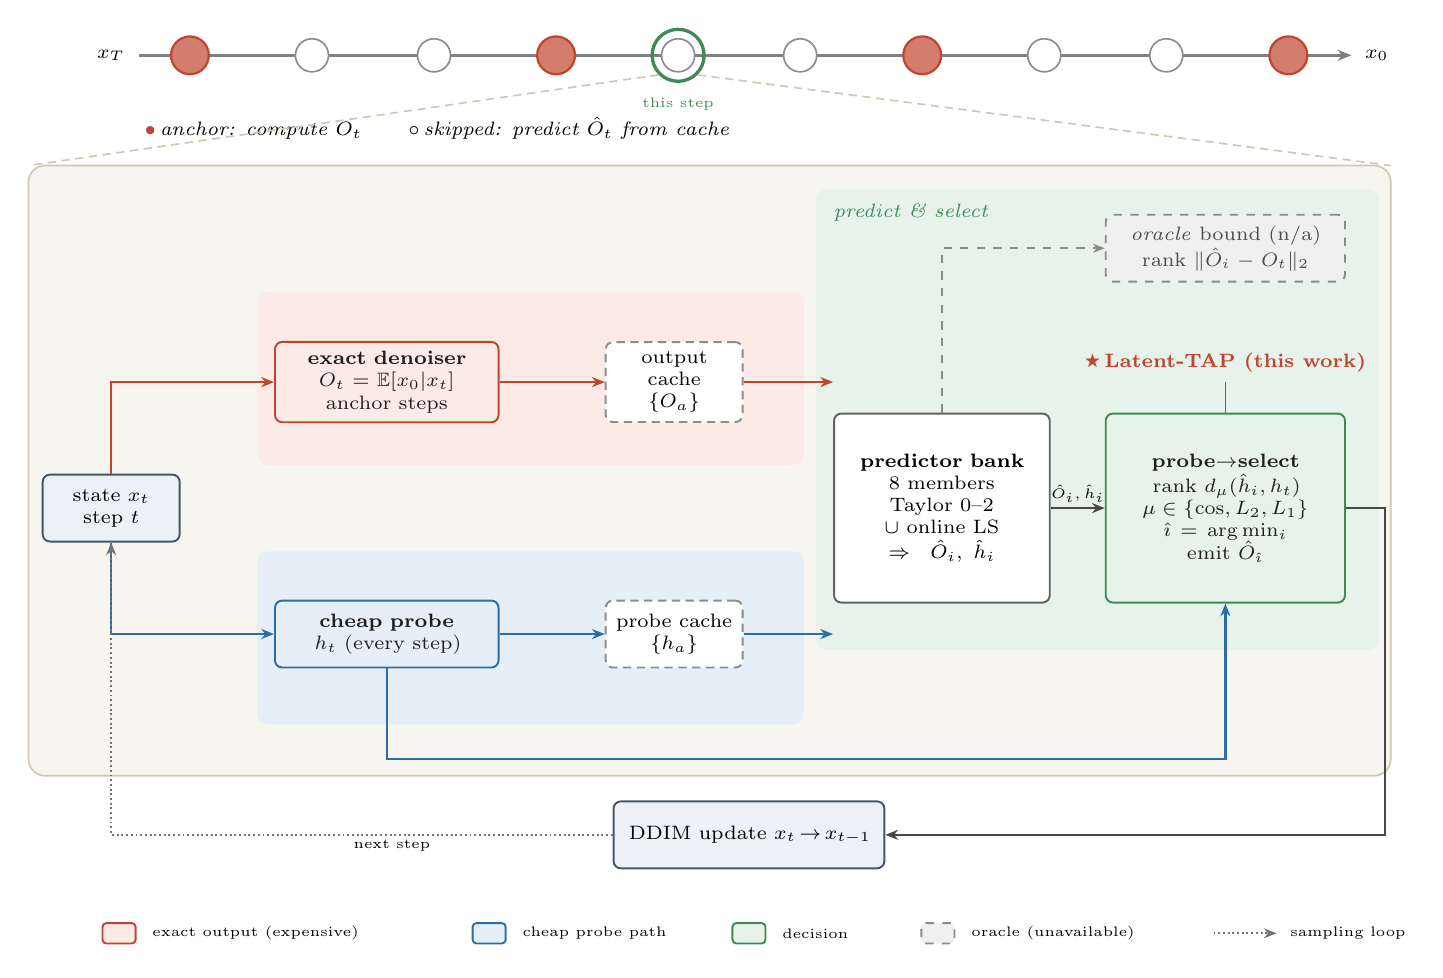
\begin{tikzpicture}[x=1cm,y=1cm]
% --- soft pastel stage panels (group logic, low saturation) ---
\begin{scope}[on background layer]
  \fill[cZone,rounded corners=6pt] (-1.05,-3.4) rectangle (16.25,4.35);
  \draw[cZoneLn,rounded corners=6pt,line width=0.6pt] (-1.05,-3.4) rectangle (16.25,4.35);
  \fill[cExpBg,rounded corners=4pt] (1.85,0.55) rectangle (8.8,2.75);
  \fill[cChpBg,rounded corners=4pt] (1.85,-2.75) rectangle (8.8,-0.55);
  \fill[cDecBg,rounded corners=4pt] (8.95,-1.8) rectangle (16.1,4.05);
  \node[cDecLn,font=\scriptsize\itshape,anchor=north west] at (9.05,3.98) {predict \& select};
\end{scope}
% --- denoising trajectory: anchors (compute) vs skipped (predict) ---
\begin{scope}[shift={(0,5.75)}]
  \draw[-{Stealth[length=5pt,width=4pt]},line width=0.9pt,black!50] (0.35,0) -- (15.75,0);
  \node[anchor=east,font=\scriptsize] at (0.3,0) {$x_T$};
  \node[anchor=west,font=\scriptsize] at (15.8,0) {$x_0$};
  \foreach \i in {0,3,6,9}{\pgfmathsetmacro\xx{1.0+\i*1.55}%
    \node[circle,draw=cExpLn,line width=0.8pt,fill=cExpLn!70,minimum size=4.8mm,inner sep=0] at (\xx,0){};}
  \foreach \i in {1,2,4,5,7,8}{\pgfmathsetmacro\xx{1.0+\i*1.55}%
    \node[circle,draw=black!45,line width=0.6pt,fill=white,minimum size=4.2mm,inner sep=0] at (\xx,0){};}
  \pgfmathsetmacro\xz{1.0+4*1.55}
  \node[circle,draw=cDecLn,line width=1.2pt,minimum size=6.6mm,inner sep=0] (zoom) at (\xz,0){};
  \node[anchor=north,font=\tiny,text=cDecLn] at (\xz,-0.42) {this step};
  \node[anchor=north west,font=\scriptsize\itshape] at (0.3,-0.66)
    {\textcolor{cExpLn}{$\bullet$}\,anchor: compute $O_t$\qquad$\circ$\,skipped: predict $\hat O_t$ from cache};
\end{scope}
% zoom-in lines from the highlighted step down onto the mechanism
\draw[cZoneLn,line width=0.6pt,densely dashed] (zoom.south west) -- (-1.05,4.35);
\draw[cZoneLn,line width=0.6pt,densely dashed] (zoom.south east) -- (16.25,4.35);
% --- nodes on a strict grid ---
\node[st,text width=15mm] (xt) at (0,0) {state $x_t$\\{\scriptsize step $t$}};
\node[exp,text width=26mm] (D) at (3.5,1.6) {\textbf{exact denoiser}\\$O_t\!=\!\mathbb{E}[x_0|x_t]$\\{\scriptsize anchor steps}};
\node[chp,text width=26mm] (h) at (3.5,-1.6) {\textbf{cheap probe}\\$h_t$ {\scriptsize (every step)}};
\node[cache,text width=15mm] (Oc) at (7.15,1.6) {output cache\\$\{O_a\}$};
\node[cache,text width=15mm] (hc) at (7.15,-1.6) {probe cache\\$\{h_a\}$};
\node[box,fill=white,draw=black!62,text width=25mm,minimum height=24mm] (bank) at (10.55,0)
   {\textbf{predictor bank}\\{\scriptsize $8$ members}\\{\scriptsize Taylor $0$–$2$}\\{\scriptsize $\cup$ online LS}\\[1pt]$\Rightarrow\ \hat O_i,\ \hat h_i$};
\node[dec,text width=28mm,minimum height=24mm] (dec) at (14.15,0)
   {\textbf{probe$\rightarrow$select}\\rank $d_\mu(\hat h_i,h_t)$\\{\scriptsize $\mu\!\in\!\{\cos,L_2,L_1\}$}\\$\hat\imath\!=\!\arg\min_i$\\emit $\hat O_{\hat\imath}$};
\node[aux,text width=28mm] (orc) at (14.15,3.3) {\emph{oracle} bound (n/a)\\rank $\|\hat O_i-O_t\|_2$};
\node[st,text width=32mm] (ddim) at (8.1,-4.15) {DDIM update\ $x_t\!\rightarrow\!x_{t-1}$};
% Latent-TAP locus marker
\node[font=\scriptsize\bfseries,text=cExpLn] (ltaptag) at (14.15,1.85) {\ding{72}\,Latent-TAP (this work)};
\draw[cExpLn,line width=0.5pt] (ltaptag.south) -- (dec.north);
% --- expensive lane (red) ---
\draw[ax] (xt.north) |- (D.west);
\draw[ax] (D) -- (Oc);
\draw[ax] (Oc.east) -- (bank.west|-Oc);
% --- cheap lane (blue) ---
\draw[ac] (xt.south) |- (h.west);
\draw[ac] (h) -- (hc);
\draw[ac] (hc.east) -- (bank.west|-hc);
% --- bank -> decision ---
\draw[a] (bank.east) -- node[above,font=\tiny,inner sep=1.6pt]{$\hat O_i,\hat h_i$} (dec.west);
% --- fresh probe h_t compared inside the decision ---
\draw[ac] (h.south) -- ++(0,-1.15) -| (dec.south);
% --- oracle taps predictors + true O_t (dashed, not deployable) ---
\draw[ad] (bank.north) |- (orc.west);
% --- selected output + sampling loop ---
\draw[a] (dec.east) -- ++(0.5,0) |- (ddim.east);
\draw[loop] (ddim.west) -| node[below,pos=0.22,font=\tiny,inner sep=1.6pt]{next step} (xt.south);
% --- legend ---
\begin{scope}[shift={(0.1,-5.4)},font=\tiny]
  \node[lgd,fill=cExpBg,draw=cExpLn] (e1) at (0,0){};    \node[anchor=west] at (0.3,0){exact output (expensive)};
  \node[lgd,fill=cChpBg,draw=cChpLn] (e2) at (4.7,0){};  \node[anchor=west] at (5.0,0){cheap probe path};
  \node[lgd,fill=cDecBg,draw=cDecLn] (e3) at (8.0,0){};  \node[anchor=west] at (8.3,0){decision};
  \node[lgd,fill=cAuxBg,draw=cAuxLn,dashed] (e4) at (10.4,0){}; \node[anchor=west] at (10.7,0){oracle (unavailable)};
  \draw[loop] (13.9,0)--(14.7,0); \node[anchor=west] at (14.75,0){sampling loop};
\end{scope}
\end{tikzpicture}}
\caption{\textbf{Architecture of the exact-residual testbed and the probe-then-select
mechanism.} Because the prior is a Gaussian mixture, the true denoiser output $O_t$ (red,
computationally expensive) is available in closed form, and a cheap hard-assignment
\emph{probe} $h_t$ (blue) plays the role of a first-layer readout. At a skipped step the
predictor bank extrapolates the cached outputs and probes; the selector ranks predictors by
a proxy distance on the probe and applies the selected predictor's output. The \emph{oracle}
(dashed) ranks by the true output error; it is not deployable and upper-bounds the gain
attainable by any proxy.}
\label{fig:arch}
\end{figure*}

\section{Introduction}
Feature-caching accelerators for diffusion transformers (DiTs)~\cite{peebles2023dit} skip
most of the network on most sampling steps and reconstruct the missing output from cached
values~\cite{ma2024deepcache,selvaraju2024fora}. The Token-Adaptive Predictor (TAP)
generalises this idea: it maintains a family of cheap extrapolators and, for each token,
selects one by reading the first-layer \emph{probe} (the modulated input) and ranking
predictors according to how closely their extrapolated probe matches the freshly computed
probe under a cosine proxy. A single-seed pilot suggested three candidate improvements:
replacing cosine with an $L_2$ proxy, replacing fixed Taylor extrapolators with online
least-squares fits, and exploiting the probe's per-token adaptivity. In this work we
evaluate these proposals under multi-seed, multi-regime testing to determine which of them
hold.

The findings are predominantly negative, and we argue that they are more informative than an
additional caching heuristic. Two of the three proposals do not survive multiple seeds, and
the third yields only a small but reproducible improvement. The study also identifies the
operative degree of freedom. Because TAP's per-token selection is separable, equal-cost, and
unconstrained, greedy per-token selection already attains the global optimum
(\S\ref{sec:theory}), so no selection-optimization gap remains. The binding constraint is
instead the fidelity of the cheap proxy to the true, unobserved output error, a quantity
that the exact testbed measures directly.

\noindent\textbf{Contributions.}
\begin{itemize}\setlength\itemsep{0.15ex}
\item An \emph{exact-residual} Gaussian-mixture diffusion testbed (Fig.~\ref{fig:arch}) in
which the true denoiser output, and therefore every predictor's true error, is closed-form,
making proxy fidelity measurable without a trained network.
\item A proof that TAP's per-token selection has \emph{zero} optimality gap, relocating the
problem from selection optimization to proxy fidelity, together with a mechanism explaining
why an $L_2$ proxy outperforms cosine.
\item A systematic evaluation ($12$-seed core, $21$-regime sweep, and a pre-registered
$30$-test suite; Fig.~\ref{fig:flow}) that retires the online-predictor and
probe-adaptivity proposals and bounds the $L_2$ improvement to a small, reproducible effect.
\end{itemize}

\section{Findings at a glance}\label{sec:findings}
We summarise the results upfront; each is established with $12$ seeds (core) or $5$
seeds per cell (sweep) and $95\%$ bootstrap CIs, and re-checked by the $30$-test suite.
\begin{enumerate}\setlength\itemsep{0.25ex}\leftskip-2pt
\item[\textbf{F1}] \textbf{The $L_2$ proxy improves on cosine in every regime, but the
effect is small.} Rank fidelity to the true error increases in \textbf{$21/21$} regimes
($\Delta$Spearman $+0.016$, CI $(+0.014,+0.019)$; top-$1$ selection accuracy $+0.028$),
rather than the roughly fourfold gain reported by the single-seed pilot. $L_1$ performs
equivalently to $L_2$, indicating that the operative factor is the use of magnitude
information rather than cosine specifically; the advantage increases with task difficulty,
from $+0.012$ at mild acceleration to $+0.034$ at cache stride $8$.
\item[\textbf{F2}] \textbf{Online least-squares predictors do not outperform fixed Taylor
extrapolators.} They are consistently worse (Taylor superior in \textbf{$19/21$} regimes,
online superior in $0/21$), and the best single fixed predictor is a Taylor extrapolator in
every regime. The advantage reported in the pilot does not replicate.
\item[\textbf{F3}] \textbf{The adaptivity of probe-then-select is beneficial only under
aggressive acceleration.} It surpasses the best fixed predictor in exactly \textbf{$1/21$}
regimes (cache stride $8$); in all milder regimes a single fixed predictor performs
comparably, so the gains attributed to adaptive caching at moderate speedups arise from the
acceleration rather than the adaptivity.
\item[\textbf{F4}] \textbf{The selection problem has no optimality gap.} Per-token
selection is separable, equal-cost, and unconstrained, so greedy selection provably attains
the global optimum (\S\ref{sec:theory}). An oracle selector nonetheless outperforms the
naive baseline (headroom $+0.005$, increasing to $+0.14$ at stride $8$), identifying
\emph{proxy fidelity}, rather than selection or the predictor family, as the binding
constraint.
\item[\textbf{F5}] \textbf{Proxy fidelity is governed by probe richness.} As the probe
ranges from a shallow hard readout to the exact output, fidelity increases monotonically
($0.33$, $0.68$, $0.73$, $1.0$). A trained DiT's learned first-layer probe lies substantially
higher on this curve (Spearman ${\approx}0.77$~\cite{challagundla2025probe}); the shallow
analytic probe used here therefore lower-bounds the effect, and the measured $L_2$ advantage
is conservative.
\item[\textbf{F6}] \textbf{Methodological.} The pre-registered $30$-test suite yields
\textbf{$26$ passes, $0$ failures, and $4$ qualifying notes}. Improvements that appear under
a single seed diminish or reverse under multi-seed evaluation, indicating that such methods
should be assessed on trained networks using paired fidelity-to-base-model metrics.
\end{enumerate}

\section{Background and related work}
\textbf{Feature caching.} DeepCache~\cite{ma2024deepcache} and FORA~\cite{selvaraju2024fora}
reuse features on fixed schedules; TeaCache~\cite{liu2024teacache} modulates reuse by a
timestep-embedding indicator; ToCa~\cite{zou2024toca} and DiCache~\cite{dicache2025} make
the decision token- or sample-adaptive; TaylorSeer~\cite{taylorseer2025} replaces
cache-and-reuse with Taylor \emph{prediction} of features. TAP generalises the predictor to
a per-token \emph{selected} member of a small family. \textbf{Diffusion samplers.} We use
the variance-preserving forward process of DDPM~\cite{ho2020ddpm} with deterministic
DDIM~\cite{song2021ddim} reverse steps; the exact posterior mean follows from
Tweedie's formula~\cite{efron2011tweedie} and the score view of
diffusion~\cite{song2019generative,song2021sde}. \textbf{Evaluation hazard.} These methods
are compared by generation quality at matched compute. A recurring hazard, which we make
explicit and which motivated the present study, is that comparisons on analytic or
untrained denoisers need not transfer to trained ones; a companion study shows that the
probe's reliability is itself an emergent property of training~\cite{challagundla2025probe}.
\textbf{Status of TAP.} TAP (arXiv:2603.03792) has no released implementation at the time
of writing. Every TAP-specific claim here rests on our faithful reconstruction of its
probe-then-select mechanism, so we evaluate the mechanism rather than a particular codebase.

\section{Positioning of Latent-TAP}\label{sec:positioning}
Training-free accelerators can be organised along two axes: the granularity of the caching
decision (a global schedule, a per-timestep gate, a per-sample gate, or a per-token gate),
and the sophistication of the reconstruction (direct feature reuse, reuse with rescaling,
Taylor forecasting, or selection from a predictor family). Figure~\ref{fig:landscape} places
representative methods in this space, and Table~\ref{tab:positioning} lists their mechanisms
together with the backbone and speedup each reports. Latent-TAP occupies the most
fine-grained and most expressive corner: it selects, per token, among a family of
extrapolators, using the first-layer probe as the gating signal. This position is shared
with TAP, which has no public implementation; the present study contributes an open
reimplementation and, more importantly, an exact testbed in which the assumptions underlying
this corner can be measured rather than assumed. Because Latent-TAP is evaluated on an
analytic denoiser, its fidelity is reported as a paired energy distance to the full sampler
(Table~\ref{tab:core}) rather than as a backbone FID; it is therefore not placed on the
speedup axis of Figure~\ref{fig:landscape}(b).

\begin{figure*}[t]\centering
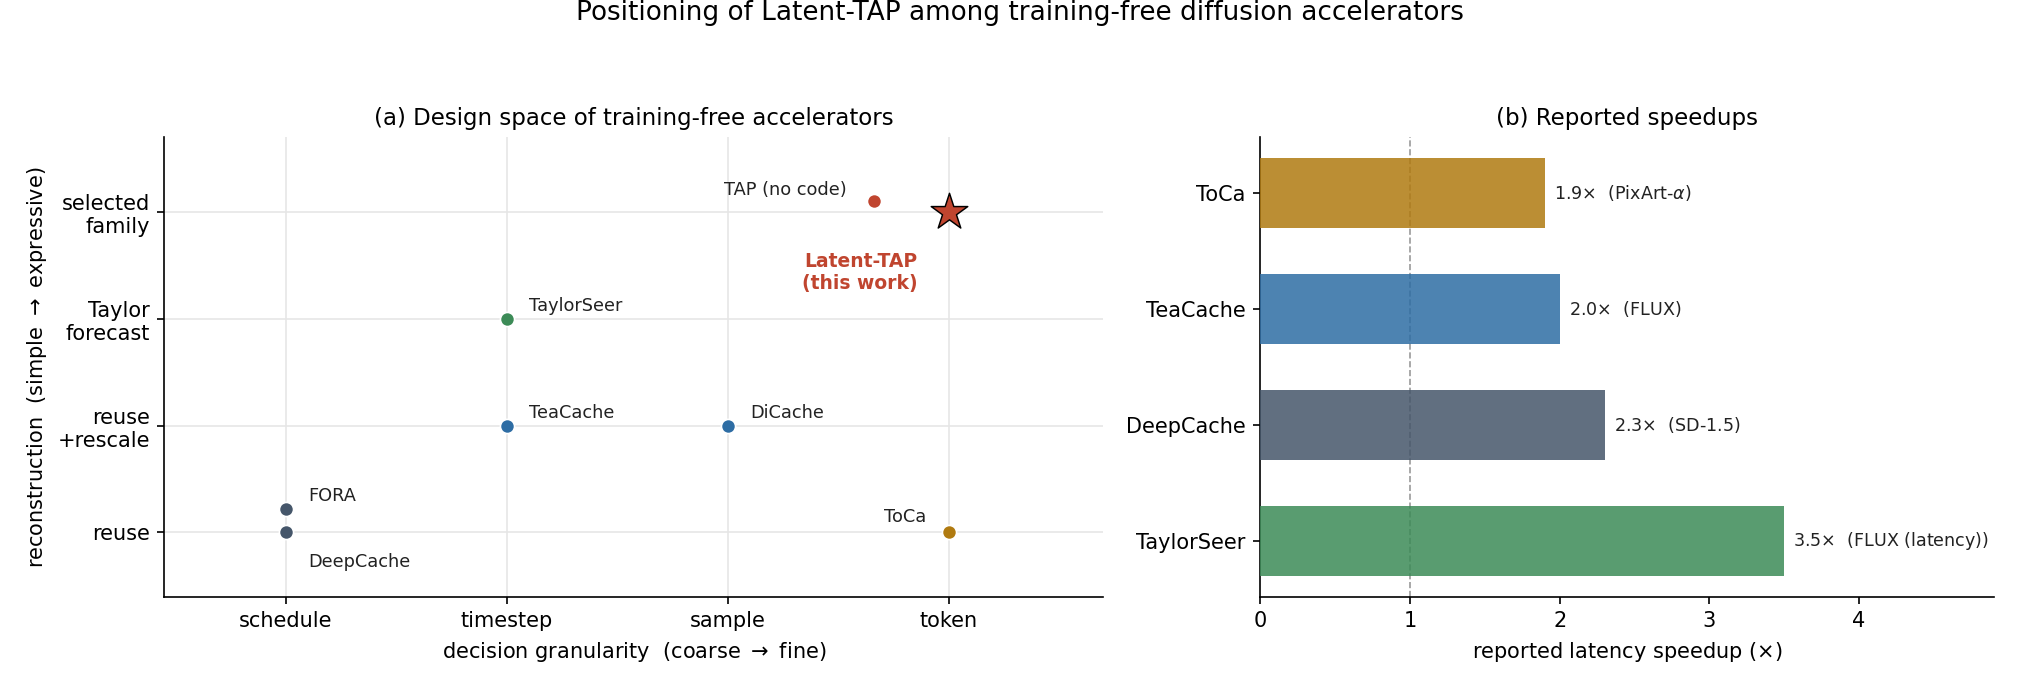
\includegraphics[width=0.99\textwidth]{fig_landscape.png}
\caption{\textbf{Positioning of Latent-TAP among training-free diffusion accelerators.}
\textbf{(a)} Design space: decision granularity (coarse to fine) against reconstruction
sophistication (simple to expressive). Latent-TAP (star) selects per token from a predictor
family, the finest and most expressive corner, a position shared with the code-less TAP.
\textbf{(b)} Latency speedups reported by each method, annotated with the backbone and
threshold at which they were obtained. These figures are drawn from the respective papers,
are not iso-quality or iso-backbone, and are shown only to situate the landscape; Latent-TAP
is evaluated on an analytic testbed and is not directly comparable, so it is omitted from
this panel.}
\label{fig:landscape}
\end{figure*}

\begin{table*}[t]\centering\footnotesize
\setlength{\tabcolsep}{5pt}
\caption{Latent-TAP relative to representative training-free diffusion accelerators.
Reconstruction, granularity, and gating signal are taken from each method's paper. Reported
speedups are latency figures at each method's own backbone and quality threshold and are
\emph{not} directly comparable; they situate the design space rather than rank methods.
$^\dagger$ reported qualitatively or setting-dependent in the source. $^\ddagger$ Latent-TAP
is evaluated on an exact-residual analytic testbed via paired energy distance to the full
sampler, so no comparable backbone speedup/FID is available.}
\label{tab:positioning}
\begin{tabular}{@{}llllcl@{}}
\toprule
Method & Reconstruction & Granularity & Gating signal & Code & Reported speedup (backbone)\\
\midrule
DeepCache~\cite{ma2024deepcache}    & reuse & schedule & fixed & \checkmark & $2.3\times$ (SD-1.5)\\
FORA~\cite{selvaraju2024fora}       & reuse & schedule & fixed interval & \checkmark & several$\times$ (DiT)$^\dagger$\\
TeaCache~\cite{liu2024teacache}     & reuse\,+\,rescale & timestep & timestep-emb.\ indicator & \checkmark & $1.5$--$2.1\times$ (FLUX, HunyuanVideo)\\
DiCache~\cite{dicache2025}          & reuse\,+\,align & sample & shallow online probe & \checkmark & state of the art$^\dagger$ (FLUX, WAN\,2.1)\\
ToCa~\cite{zou2024toca}             & reuse (token) & token & token-selection scores & \checkmark & $1.5$--$2.4\times$ (PixArt-$\alpha$, OpenSora)\\
TaylorSeer~\cite{taylorseer2025}    & Taylor forecast & timestep & fixed order & \checkmark & $3.5\times$ latency (FLUX)\\
TAP~\cite{tap2026}                  & selected family & token & first-layer probe (cosine) & \ding{55} & --- (no public code)\\
\rowcolor{black!8}
\textbf{Latent-TAP} (this work)     & selected family & token & first-layer probe ($L_2$/cos) & \checkmark & analytic testbed$^\ddagger$\\
\bottomrule
\end{tabular}
\end{table*}

\section{The exact-residual testbed}\label{sec:testbed}
Proxy fidelity cannot be measured directly on a trained network, since computing the true
skipped output would negate the acceleration it is intended to provide. We therefore adopt a
prior for which the exact denoiser is available in closed form. Data are drawn from a
$K$-component isotropic Gaussian
mixture in $\mathbb R^d$; under the variance-preserving forward process $x_t=\sqrt{\bar
\alpha_t}\,x_0+\sqrt{1-\bar\alpha_t}\,\varepsilon$ the posterior mean is exactly
\begin{equation}
O_t \equiv \mathbb E[x_0\mid x_t]=\sum_{k=1}^{K} r_k(x_t,t)\,\big[\mu_k+c_t\,(x_t-\sqrt{\bar\alpha_t}\mu_k)\big],
\end{equation}
with responsibilities $r_k\!\propto\! w_k\,\mathcal N\!\big(x_t;\sqrt{\bar\alpha_t}\mu_k,(\bar\alpha_t\sigma^2{+}1{-}\bar\alpha_t)I\big)$
and $c_t=\sqrt{\bar\alpha_t}\sigma^2/(\bar\alpha_t\sigma^2{+}1{-}\bar\alpha_t)$. This
constitutes the computationally expensive output. The cheap \emph{probe} $h_t$ is the
hard-assignment denoiser, retaining only the $\arg\max_k r_k$ term; it serves as the
analogue of a shallow first-layer readout operating on an approximate rather than exact
decision. Tokens are i.i.d.\ draws sharing the mixture, and DDIM steps use $O$ at anchor
steps and a predicted $\hat O$ at skipped steps (Fig.~\ref{fig:arch}).

\textbf{Predictors.} A family of $8$: fixed finite-difference Taylor extrapolators of order
$0$--$2$ at horizons $1$--$2$, plus online least-squares fits (degree $2$--$3$ over windows
of $5$--$6$ anchors). \textbf{Proxy-then-select.} Each predictor extrapolates the cached
outputs ($\hat O_i$) and cached probes ($\hat h_i$); the selector picks per token
$\hat\imath=\arg\min_i d_\mu(\hat h_i,h_t)$ for proxy $\mu\in\{\cos,L_2,L_1\}$ and applies
$\hat O_{\hat\imath}$. \textbf{Oracle} instead minimises the true error $\|\hat
O_i-O_t\|_2$. \textbf{Metrics.} (a) the rank correlation between proxy error and true error
across the predictor family, which measures whether the proxy orders the predictors
correctly; and (b) the energy distance~\cite{szekely2013energy} between the accelerated and
full samplers' final samples, which measures end-to-end distributional fidelity. We use
$12$ seeds for the core study and $5$ per regime cell, with bootstrap $95\%$ confidence
intervals throughout.

\section{Optimality of greedy per-token selection}\label{sec:theory}
Let $f_n(i)$ be the true reconstruction error of predictor $i$ on token $n$ at a skipped
step. TAP minimises $\sum_n f_n(\pi_n)$ over assignments $\pi$. Three properties hold: the
objective is \emph{separable} (token $n$'s cost depends only on $\pi_n$), the choices are
\emph{equal-cost} (every predictor is one cheap extrapolation; no shared budget), and the
feasible set is a \emph{product} set. Hence
\begin{equation}
\min_{\pi}\ \sum_{n} f_n(\pi_n)\;=\;\sum_n \min_i f_n(i),
\end{equation}
so greedy per-token selection attains the global optimum. A regret bound or knapsack
formulation over the joint assignment therefore addresses a problem with no optimality gap,
which was the error in the pilot's original framing. The relevant regret is not
combinatorial but statistical: the true errors $f_n(i)$ are never observed; instead we
observe a proxy $g_n(i)=d_\mu(\hat
h_i,h)$ and deploy $\hat\pi_n=\arg\min_i g_n(i)$. The excess error $\mathbb E[f_n(\hat
\pi_n)-\min_i f_n(i)]$ is governed entirely by the rank agreement between $g$ and $f$. The
quantities that can reduce this excess error are a more informative metric $\mu$ or a richer
probe $h$.

\textbf{Why $L_2$ tracks the residual more faithfully than cosine.} The true error is an
$L_2$ residual $\|\hat O_i-O\|_2$, whereas cosine measures only the angle and discards
magnitude, $d_{\cos}=1-\langle\hat h_i,h\rangle/(\|\hat h_i\|\,\|h\|)$. When predictors
differ mainly in the degree to which they over- or under-shoot, which is the dominant
failure mode as the extrapolation horizon grows, the discriminating signal is radial;
cosine is insensitive to this component, whereas $L_2$ and $L_1$ retain it. When the
probe-to-output map is locally affine near the anchors, magnitude ordering is approximately
preserved, and the $L_2$ proxy is the better-aligned surrogate. This account predicts that
the $L_2$ advantage should increase with acceleration and noise, both of which enlarge the
radial error, a prediction the sweep confirms (\S\ref{sec:sweep}). We present this as a
mechanism rather than a theorem; the corresponding inequality holds empirically in all $21$
regimes.

% =========================== WORKFLOW DIAGRAM ===========================
\begin{figure*}[t]\centering
\resizebox{\textwidth}{!}{%
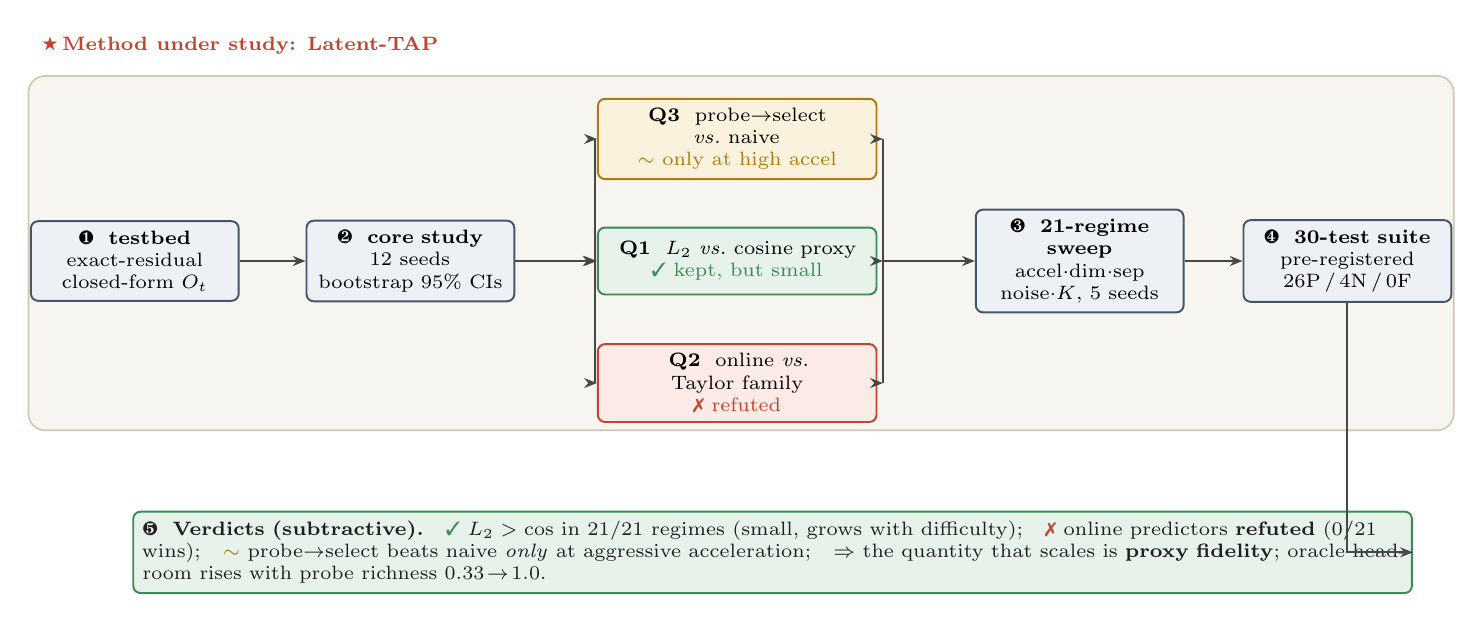
\begin{tikzpicture}[x=1cm,y=1cm]
% --- soft backdrop band behind the pipeline row ---
\begin{scope}[on background layer]
  \fill[cZone,rounded corners=6pt] (-1.35,-2.15) rectangle (16.75,2.35);
  \draw[cZoneLn,rounded corners=6pt,line width=0.6pt] (-1.35,-2.15) rectangle (16.75,2.35);
\end{scope}
\node[font=\scriptsize\bfseries,text=cExpLn,anchor=south west] at (-1.3,2.5) {\ding{72}\,Method under study: Latent-TAP};
% --- numbered stages ---
\node[st,text width=24mm] (tb)   at (0,0)     {\textbf{\ding{182}\ \ testbed}\\{\scriptsize exact-residual}\\{\scriptsize closed-form $O_t$}};
\node[st,text width=24mm] (core) at (3.5,0)   {\textbf{\ding{183}\ \ core study}\\{\scriptsize $12$ seeds}\\{\scriptsize bootstrap $95\%$ CIs}};
% --- three questions, tinted by outcome ---
\node[box,fill=cAmbBg,draw=cAmbLn,text width=33mm] (q3) at (7.65,1.55)  {\textbf{Q3}\ \ probe$\rightarrow$select \emph{vs.}\ naive\\{\scriptsize\textcolor{cAmbLn}{$\sim$ only at high accel}}};
\node[box,fill=cDecBg,draw=cDecLn,text width=33mm] (q1) at (7.65,0)     {\textbf{Q1}\ \ $L_2$ \emph{vs.}\ cosine proxy\\{\scriptsize\textcolor{cDecLn}{\ding{51} kept, but small}}};
\node[box,fill=cExpBg,draw=cExpLn,text width=33mm] (q2) at (7.65,-1.55) {\textbf{Q2}\ \ online \emph{vs.}\ Taylor family\\{\scriptsize\textcolor{cExpLn}{\ding{55} refuted}}};
\node[st,text width=24mm] (sweep) at (12.0,0) {\textbf{\ding{184}\ \ 21-regime sweep}\\{\scriptsize accel$\cdot$dim$\cdot$sep}\\{\scriptsize noise$\cdot K$, $5$ seeds}};
\node[st,text width=24mm] (pt)    at (15.4,0) {\textbf{\ding{185}\ \ 30-test suite}\\{\scriptsize pre-registered}\\{\scriptsize $26$P\,/\,$4$N\,/\,$0$F}};
% --- verdict panel with matching glyphs ---
\node[dec,align=left,text width=160mm] (v) at (8.1,-3.7)
  {\textbf{\ding{186}\ \ Verdicts (subtractive).}\quad
   \textcolor{cDecLn}{\ding{51}}~$L_2\!>\!\cos$ in \textbf{$21/21$} regimes (small, grows with difficulty);\quad
   \textcolor{cExpLn}{\ding{55}}~online predictors \textbf{refuted} (\textbf{$0/21$} wins);\quad
   \textcolor{cAmbLn}{$\sim$}~probe$\rightarrow$select beats naive \emph{only} at aggressive acceleration;\quad
   $\Rightarrow$ the quantity that scales is \textbf{proxy fidelity}; oracle headroom rises with probe richness $0.33\!\rightarrow\!1.0$.};
% --- fan-out bus: core -> Q1/Q2/Q3 ---
\draw[a] (core.east) -- (5.85,0);
\draw[black!72,line width=0.7pt] (5.85,-1.55) -- (5.85,1.55);
\draw[a] (5.85,1.55) -- (q3.west);
\draw[a] (5.85,0)    -- (q1.west);
\draw[a] (5.85,-1.55)-- (q2.west);
% --- fan-in bus: Q* -> sweep ---
\draw[a] (q3.east) -- (9.5,1.55);
\draw[a] (q1.east) -- (9.5,0);
\draw[a] (q2.east) -- (9.5,-1.55);
\draw[black!72,line width=0.7pt] (9.5,-1.55) -- (9.5,1.55);
\draw[a] (9.5,0) -- (sweep.west);
% --- sequential + hand-off to verdicts ---
\draw[a] (tb) -- (core);
\draw[a] (sweep) -- (pt);
\draw[a] (pt.south) |- (v.east);
\end{tikzpicture}}
\caption{\textbf{Experimental workflow.} The exact testbed feeds a $12$-seed core study
that isolates three questions (Q1--Q3); each is then stress-tested across a $21$-regime
sweep and a pre-registered $30$-test adversarial suite. Every comparison is paired and
bootstrapped. The overall conclusion is negative: only the $L_2$ proxy holds, and it is
small; the operative quantity is proxy fidelity, determined by probe richness.}
\label{fig:flow}
\end{figure*}

\begin{table}[t]\centering\small
\caption{Core study ($12$ seeds, stride-$3$ base regime). Energy distance to the full
sampler (lower is better); paired differences with $95\%$ bootstrap CIs.}
\label{tab:core}
\begin{tabular}{lcc}
\toprule
quantity & value & paired CI\\
\midrule
proxy Spearman, cosine & 0.315 & \textit{ref.}\\
proxy Spearman, $L_2$ & 0.331 & $+0.016\,(+.014,+.019)$\\
top-1 pick acc, cosine & 0.393 & \textit{ref.}\\
top-1 pick acc, $L_2$ & 0.421 & $+0.028\,(+.024,+.032)$\\
\midrule
energy: Taylor family & 0.0210 & \textit{ref.}\\
energy: online family & 0.0249 & $-0.004\,(-.006,-.002)$\\
\midrule
energy: random select & 0.0281 & \textit{ref.}\\
energy: naive best-fixed & 0.0164 & \textit{ref.}\\
energy: probe-then-select & 0.0207 & $+0.004\,(+.002,+.006)$\\
energy: oracle & 0.0112 & $-0.005\,(-.007,-.003)$\\
\bottomrule
\end{tabular}
\end{table}

\section{Core results}\label{sec:core}
Table~\ref{tab:core} summarises the core study. The $L_2$ proxy improves rank fidelity and
top-$1$ selection accuracy over cosine; the difference is statistically reliable (the
confidence interval excludes zero) but modest, amounting to a $5\%$ relative gain in
Spearman correlation rather than the roughly fourfold gain suggested by the single-seed
pilot. $L_1$ performs equivalently to $L_2$, confirming that the improvement derives from
the use of magnitude information rather than from cosine specifically. The
online-least-squares family is consistently worse than fixed Taylor, and combining the two
families does not improve on Taylor alone. Probe-then-select is outperformed by the best
fixed predictor in this setting ($+0.004$ in energy distance), yet the oracle selector
clearly outperforms the naive baseline ($-0.005$): the headroom is genuine, but the probe
proxy is too weak to realise it. The limiting factor is therefore proxy fidelity, not the
predictor family or the selection rule.

\begin{figure*}[t]\centering
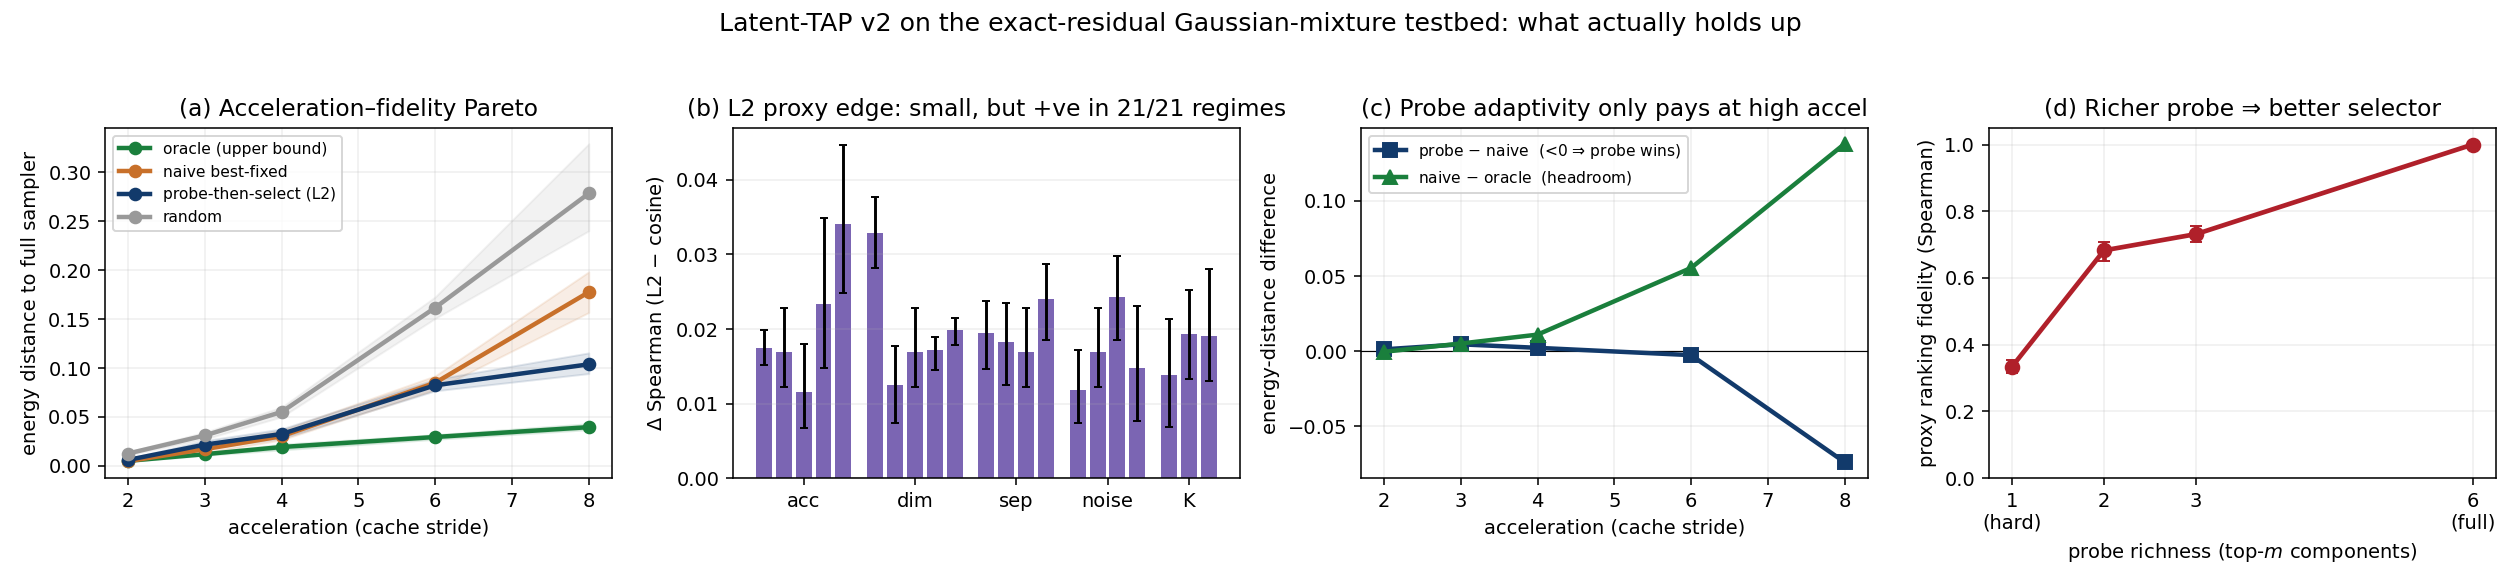
\includegraphics[width=0.98\textwidth]{fig_v2.png}
\caption{\textbf{(a)} Acceleration--fidelity trade-off: probe-then-select tracks the naive
best-fixed predictor until high stride, where it separates toward the oracle.
\textbf{(b)} The $L_2$ proxy advantage over cosine is small but positive in all $21$
regimes, widening with acceleration and noise. \textbf{(c)} Probe adaptivity is beneficial
only at aggressive acceleration (probe$-$naive crosses below $0$ at stride $8$), where the
selection headroom (naive$-$oracle) is largest. \textbf{(d)} Proxy fidelity increases
monotonically with probe richness, from a shallow hard probe ($0.33$) to the full output
($1.0$); this is the axis along which a trained DiT probe would improve.}
\label{fig:v2}
\end{figure*}

\section{Sensitivity across regimes}\label{sec:sweep}
We vary acceleration (cache stride $2$ to $8$), dimension ($2$ to $32$), mixture separation,
noise scale, and component count $K$, giving $21$ regimes with $5$ seeds each
(Fig.~\ref{fig:v2}). \textbf{The $L_2$ advantage is universal but small.} It is positive and
significant in all $21$ regimes, increasing from $+0.012$ at mild settings to $+0.034$ at
stride $8$ and $+0.024$ at high noise, consistent with the radial-error mechanism.
\textbf{Online predictors never win.} Taylor is significantly better in $19/21$ regimes and
online in none; the best single fixed predictor is a Taylor extrapolator in every regime.
\textbf{Probe adaptivity is confined to the aggressive-acceleration regime.}
Probe-then-select outperforms the naive best-fixed predictor in exactly one regime, stride
$8$, where fixed extrapolation degrades sufficiently that per-token switching becomes
worthwhile (probe$-$naive $=-0.074$). In all milder regimes the two curves coincide
(Fig.~\ref{fig:v2}a), so the gains of adaptive caching at moderate speedups are attributable
to the acceleration rather than the adaptivity. Selection headroom increases with
acceleration (Fig.~\ref{fig:v2}c), so the aggressive regimes are precisely those in which a
better proxy would be most valuable. \textbf{Proxy fidelity is the operative factor.}
Replacing the shallow hard probe with a richer top-$m$ soft readout increases rank fidelity
monotonically, from $0.33$ to $0.68$, $0.73$, and $1.0$ (Fig.~\ref{fig:v2}d). A trained
DiT's learned first-layer probe lies substantially higher on this curve (our companion study
measures Spearman ${\approx}0.77$~\cite{challagundla2025probe}), so the testbed lower-bounds
the probe's value and the measured $L_2$ advantage is a conservative estimate.

\section{Adversarial test suite}
We pre-registered $30$ tests, each designed to falsify a claim: testbed-correctness checks
(exact-denoiser limits, $\mathrm{energy}(\text{full},\text{full}){=}0$, and absence of
true-error leakage into selection), the multi-seed core comparisons, the $21$-regime
crossovers, monotonicity of the acceleration--fidelity trade-off, monotonicity of a
budget/abstaining selector in the compute--fidelity plane, and the probe-richness curve. The
suite yields \textbf{$26$ passes, $0$ failures, and $4$ qualifying notes}: the $L_2$
improvement is small rather than fourfold; the absolute proxy Spearman correlation is only
moderate; the end-to-end quality gain of $L_2$ over cosine at the selection level is
negligible; and at mild acceleration the acceleration, not the adaptivity, accounts for the
measured gains. No test designed to falsify a surviving claim succeeded, and the two retired
proposals failed precisely the tests intended to detect them.

\section{Discussion}
The results are predominantly negative. Of the three proposed improvements to a
token-adaptive predictor, one (online predictors) provides no benefit, one (probe
adaptivity) is beneficial only in the aggressive-acceleration regime, and one (the $L_2$
proxy) yields a small but reliable improvement attributable to the use of magnitude
information. These observations are unified by the fact that TAP's selection is already
optimal given the true errors, so the operative quantity is proxy fidelity, determined by
the choice of metric and, to a greater extent, by the richness of the probe. This reframes
the problem from method tuning to measurement, which the exact-residual testbed makes
tractable.

\section{Limitations}
The denoiser is an analytic Gaussian mixture rather than a trained network, and the probe is
a shallow hard-assignment readout. Both choices ensure that the ground truth is computable,
but both render the probe a weaker ranker than a trained DiT's learned first layer
(Fig.~\ref{fig:v2}d and \cite{challagundla2025probe}). The absolute energy-distance
magnitudes are testbed-specific, so all conclusions rely on paired, within-regime
comparisons. TAP provides no public code, so we evaluate the mechanism rather than a
reference implementation. Whether the small $L_2$ advantage and the aggressive-acceleration
probe benefit increase or diminish on large latent DiTs remains open and requires
computational resources beyond those used here.

\section{Conclusion}
We evaluated three proposed improvements to a training-free diffusion predictor and found
that most do not hold. Under multi-seed, multi-regime testing, online predictors do not
outperform fixed Taylor extrapolators, probe adaptivity is beneficial only at aggressive
acceleration, and the $L_2$ proxy provides a small but reliable improvement over cosine
because it retains the magnitude information on which the true residual depends. Since
per-token selection is provably optimal, the only quantity that scales is proxy fidelity,
which is determined by the metric and, to a greater extent, by the richness of the probe.
We recommend that such methods be evaluated on trained networks using
fidelity-to-base-model metrics, and that the probe, rather than the selection rule, be the
primary target for improvement.

{\small\textbf{Reproducibility.} All code and results run locally in pure NumPy:
\code{latap\_v2.py} (testbed), \code{run\_core.py}/\code{agg\_core.py} ($12$-seed core),
\code{sweep.py}/\code{sweep\_agg.py} ($21$-regime sweep), \code{probe\_depth.py}
(richness), \code{pressure\_v2.py} ($30$-test suite), \code{plot\_v2.py}; data in
\code{results/}. See the repository \textsc{readme} for exact commands.}

\begin{thebibliography}{99}\small
\bibitem{ho2020ddpm} J.~Ho, A.~Jain, P.~Abbeel. Denoising Diffusion Probabilistic Models. \emph{NeurIPS}, 2020.
\bibitem{song2021ddim} J.~Song, C.~Meng, S.~Ermon. Denoising Diffusion Implicit Models. \emph{ICLR}, 2021.
\bibitem{song2019generative} Y.~Song, S.~Ermon. Generative Modeling by Estimating Gradients of the Data Distribution. \emph{NeurIPS}, 2019.
\bibitem{song2021sde} Y.~Song et al. Score-Based Generative Modeling through Stochastic Differential Equations. \emph{ICLR}, 2021.
\bibitem{peebles2023dit} W.~Peebles, S.~Xie. Scalable Diffusion Models with Transformers. \emph{ICCV}, 2023.
\bibitem{efron2011tweedie} B.~Efron. Tweedie's Formula and Selection Bias. \emph{JASA}, 106(496), 2011.
\bibitem{szekely2013energy} G.~J.~Sz\'ekely, M.~L.~Rizzo. Energy Statistics: A Class of Statistics Based on Distances. \emph{J.\ Stat.\ Plan.\ Inference}, 2013.
\bibitem{ma2024deepcache} X.~Ma, G.~Fang, X.~Wang. DeepCache: Accelerating Diffusion Models for Free. \emph{CVPR}, 2024.
\bibitem{selvaraju2024fora} P.~Selvaraju et al. FORA: Fast-Forward Caching in Diffusion Transformer Acceleration. arXiv:2407.01425, 2024.
\bibitem{liu2024teacache} F.~Liu et al. Timestep Embedding Tells: It's Time to Cache for Video Diffusion Models (TeaCache). arXiv:2411.19108, 2024.
\bibitem{zou2024toca} C.~Zou et al. Accelerating Diffusion Transformers with Token-wise Feature Caching (ToCa). arXiv:2410.05317, 2024.
\bibitem{dicache2025} DiCache: Learning a Shallow-Layer Online Probe for Adaptive Diffusion Caching. arXiv:2508.17356, 2025.
\bibitem{taylorseer2025} TaylorSeer: From Reusing to Forecasting---Accelerating Diffusion Transformers with Taylor Prediction. arXiv:2503.06923, 2025.
\bibitem{challagundla2025probe} B.~C.~Challagundla. Probe Reliability is an Emergent Property of Trained Diffusion Models. Companion technical report, 2025.
\bibitem{tap2026} Token-Adaptive Predictor for Training-Free Diffusion Acceleration. arXiv:2603.03792 (no public code; reimplemented here).
\end{thebibliography}

\end{document}
